\documentclass{beamer} 
\usetheme{default} 
\setbeamercovered{transparent}

%\useoutertheme{umbcfootline} 
\setbeamertemplate{background canvas}[vertical shading][bottom=red!20,top=yellow!30] 


%\usepackage[spanish]{babel}
%\usepackage[latin1]{inputenc}
\usepackage[utf8x]{inputenc}
\usepackage{multicol}


\title{XML}

\author{Manuel J. Molino Milla \and Luis Molina Garzón}

\date{\today} %

\institute{IES Virgen del Carmen \and Departamento de Informática}




%\beamerdefaultoverlayspecification{<+->}

\begin{document}


\begin{frame}
  \titlepage
\end{frame}

\begin{frame}
    \frametitle{Logo}
\begin{figure}

\includegraphics[scale=1]{imagenes/logo.jpeg} 
\caption{Logo Java}
\end{figure}
\end{frame}

\begin{frame}
  \frametitle{Contenido}
  \tableofcontents[pausesections]
\end{frame}



\section{INTRODUCCIÓN}


\begin{frame}[fragile]
\frametitle{XML}
\begin{itemize}[<+->]
\item \alert{XML} es un lenguaje de marcas que permite categorizar y organizar información.
\item Se desarrolló en 1996 bajo los auspicios del consorcio \emph{WWW}
\item Como lenguaje de marcas usa \emph{tags} para contener dicha información.
\item Ejemplo:
\end{itemize}
\begin{verbatim}
<instituto>
  <departamento>
    <nombre>Informática</nombre>
    <numeroMiembros>16</numeroMiembros>
  </departamento>
  <departamento>
    <nombre>Comercio</nombre>
    <numeroMiembros>10</numeroMiembros>
  </departamento>
</instituto>
  \end{verbatim}
\end{frame}

\begin{frame}[fragile]
\frametitle{XML}
Podemos usar atributos para describir la estructura del archivo XML:
\begin{verbatim}
<instituto>
  <departamento nombre="Informática"
                numeroMiembros="16" />
  <departamento nombre="Comercio"
                numeroMiembros="10" />
</instituto>
\end{verbatim}
\end{frame}



\section{API JAVA PARA XML}
\begin{frame}
\frametitle{Leer y parsear contenido XML} 

\begin{itemize}[<+-| alert@+>]
      \item Java posee varias API para analizar archivos XML.
      \item Una de ellas es \emph{SAX} acrónimo de \emph{Simple API for XML }.
      \item Nos sirve tanto para leer o escribir ficheros XML.
     \item Es un protocolo usado por \emph{servlets} y programas orientado a la red para transmitir y recibir documentos XML, al ser rápido y consume poca memoria.
      \item No construye una representación interna del documento como en el caso de otra API que es \emph{DOM}
      \item Se suele usar la interfaz \emph{ContentHandler} que implementa métodos como \alert{startDocument, endDocument, startElement, y endElement.}
      \begin{description}
      \item[startDocument():] Recibe notificación del principio de documento.
      \item[endDocument():] Recibe notificación del fin de documento.
      \item[startElement(String name, AttributeList atts):] Recibe notificación del principio de un elemento.
      \item[endElement(String name):] Recibe notificación del fin de elemento.
      \end{description}
      \end{itemize}
\end{frame}

\subsection{SAX}
\begin{frame}[fragile]
\frametitle{Analizando ficheros XML}
Antes de usar la interfaz anterior debemos crear un objeto \emph{SAXParseFactory} para poder crear un objeto \emph{SAXParser}
\begin{verbatim}
static public void main(String[] args) throws Exception {

    // ...

    SAXParserFactory spf = SAXParserFactory.newInstance();
    spf.setNamespaceAware(true);
    SAXParser saxParser = spf.newSAXParser();
    
    //Parseamo un fichero
    saxParser.parse("fichero.xml", new XMLHander();
    
    // XMLHandler será una clase que extienda 
    // de ContentHandler
}
\end{verbatim}
\end{frame}

\begin{frame}[fragile]
\frametitle{Analizando fichero XML}
Posteriormente debemos crear el manejador de los ficheros, se implementan algunos métodos como \emph{startElement, endElement, \dots}
\begin{scriptsize}

\begin{verbatim}
public class SAXLocalNameCount extends DefaultHandler {
      private Hashtable tags;
      public void startDocument() throws SAXException {
        tags = new Hashtable();
    	  }
    	  public void startElement(String namespaceURI,
                         String localName,
                         String qName, 
                         Attributes atts)
        throws SAXException {
          String key = localName;
          Object value = tags.get(key);
          if (value == null) {
            tags.put(key, new Integer(1));
          } 
          else {
            int count = ((Integer)value).intValue();
            count++;
            tags.put(key, new Integer(count));
          }
      }
      .............
\end{verbatim}

\end{scriptsize}
\end{frame}

\subsection{DOM}
\begin{frame}
\frametitle{DOM}
\begin{itemize}[<+->]
\item \alert{DOM} acrónimo de \emph{Document Object Model}
\item Es una estructura de árbol donde cada nodo contiene información acerca del documento XML.
\item Los dos mas comunes tipos de nodos son los \emph{nodo elemento} y los \emph{nodo texto}
\item DOM define las siguientes interfaces de objetos XML:
\begin{description}
\item[Document] Proporciona información del documento. Permite crear nuevos nodos en el documento.
\item[Element] Expone propiedades y métodos para manipular los elementos del documento y sus atributos.
\item[Node] Representa a cualquier nodo del documento.
\item[NodeList] Colección de nodos a los que se puede acceder por medio de un índice.
\item[Attr] Permite acceder a los atributos de un nodo.
\item[CharacterData] Proporciona atributos y métodos para manipular los datos de caracteres.
\end{description} 
\end{itemize}
\end{frame}

\begin{frame}
\frametitle{Interfaz Node}
\begin{description}[<+->]
\item[childNodes] lista de los nodos secundarios.
\item[firstChild] primer nodo secundario.
\item[lastChild] último nodo secundario.
\item[nextSibling] siguiente nodo similar.
\item[previousSibling] nodo previo similar.
\item[parentNode] nodo padre actual.
\item[nodeName] nombre del nodo.
\item[nodeType] tipo de nodo DOM XML. 1 Elemento, 2 Atributo, 3 Texto\dots
\item[nodeValue] valor del nodo. En el caso de un Elemento, su valor es null. Para un atributo será el valor del atributo.
\item[hasChildNodes()] indica si tiene nodos secundarios.
\item[getElementsByTagName()] Lista de nodos con elementos de un tipo.
\end{description}
\end{frame}

\begin{frame}
\frametitle{Crear documentos XML}
\begin{scriptsize}

\begin{block}{Iterfaz Document}
\begin{itemize}[<+->]
\item \alert{createElement(nombre)} Crea un nuevo elemento a partir de su nombre, devuelve el objeto Element.
\item \alert{createAtribute(nombre)} Crea un objeto Atrr con nombre.
createTextNode(cadena). Crea un nodo de texto a partir de la cadena.
\item \alert{createTextNode(cadena)} Crea un nodo de texto a partir de la cadena.
\end{itemize}
\end{block}

\begin{block}{Interfaz Node}
\begin{itemize}[<+->]
\item \alert{insertBefore(nodo,referencia)} Inserta el nodo pasado como parámetro, antes del nodo secundario de referencia. Devuelve el nodo añadido.
\item \alert{appendChild(nodo)} Añade el nuevo nodo al final de los demás nodos secundarios. Si ya existe en el árbol será eliminado de donde está.
\item \alert{replaceChild(nodo,referencia)} Sustituye el nodo secundario de referencia por el nuevo nodo. Devuelve una copia del nodo sustituido. 
\item \alert{removeChild(referencia)} Elimina el nodo indicado.
\item \alert{cloneNode(modo)} Devuelve un duplicado del nodo. Si modo es true,
clonará también los nodos descendentes, si es false solo clonará al propio nodo.
\end{itemize}
\end{block}

\end{scriptsize}
\end{frame}

\begin{frame}[fragile]
\frametitle{Ejemplo}
\begin{scriptsize}
\begin{verbatim}
public class Test3XML {

  public static void main(String[] args) {
   DocumentBuilderFactory dbf = DocumentBuilderFactory.newInstance();
   DocumentBuilder db;
   try {
    //Parse el XML instituto2.xml
       db = dbf.newDocumentBuilder();
       Document doc = db.parse(new File("instituto2.xml"));
       Element raiz = doc.getDocumentElement();
       //creo una lista con aquellas etiquetas denominada nombre
       NodeList list = raiz.getElementsByTagName("nombre");

       //recorro la lista anterior 
       for (int i = 0; i < list.getLength(); i++) {
         System.out.println(list.item(i).getFirstChild().getNodeValue());
       }
			
   } catch (ParserConfigurationException | SAXException | IOException e) {
       // TODO Auto-generated catch block
       e.printStackTrace();
   } 
  }
}
\end{verbatim}
\end{scriptsize}
\end{frame}

\section{PATRONES DE DISEÑO EN JAVA}
\begin{frame}
\frametitle{Introducción}
\begin{itemize}[<+->]
\item Los patrones de diseño son la base para la búsqueda de soluciones a problemas comunes en el desarrollo de software.
\item Proporciona catálogos de elementos reusables en el diseño de sistemas software.
\item Evitar la reiteración en la búsqueda de soluciones a problemas ya conocidos y solucionados anteriormente.
\item Estandariza el modo en que se realiza el diseño.
\item Facilita el aprendizaje de las nuevas generaciones de diseñadores condensando conocimiento ya existente.
\item Permiten hablar un lenguaje común entre un equipo de desarrollo.
\item En resumen, son soluciones simples y elegantes a problemas específicos del diseño de software orientado a objetos.
\end{itemize}
\end{frame}

\subsection{Patrón singleton}
\begin{frame}
\frametitle{Patrón Singleton }
\begin{scriptsize}

\begin{itemize}[<+->]
\item También se conoce como Instancia única
\item Su objetivo es restringir la creación de objetos  pertenecientes a una clase.
\item Evitarç la reiteración en la búsqueda de soluciones a problemas ya conocidos y solucionados anteriormente.
\item De modo que solo se tenga una única instancia de la clase para toda la aplicación, garantizando así un punto de acceso global al objeto creado. 
\item Para implementarlo, la clase Singleton debe tener un constructor privado que solo sera accedido desde la misma clase.
\item Se crea también una instancia privada de la clase, así como un método estático que permita el acceso a dicha instancia de la forma \alert{ClaseSingleton.getInstanciaSingleton();}
\item Es  muy útil cuando necesitamos crear un clase común y global para todo el sistema, donde no nos interese crear varias instancias de la misma.
\item Ejemplo una clase conexión a una BD, o a un \emph{scanner}, o la carga de los datos de un archivo de propiedades.

\end{itemize}

\end{scriptsize}
\end{frame}

\begin{frame}
\begin{figure}
\frametitle{UML singleton}
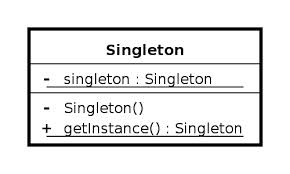
\includegraphics[scale=0.8]{imagenes/singleton.jpg}
\end{figure}
\end{frame}

\begin{frame}[fragile]
\frametitle{Código singleton}
\begin{scriptsize}

\begin{verbatim}
public class SingletonExample {

    //Instancia privada del objeto
    private static SingletonExample singletonInstance;

    // Previene solo se cree una única instancia
    // del objeto, al ser constructor privado
    private SingletonExample() {
	}

    // Acceso desde fuera
    public static SingletonExample getSingletonInstance() {
      if (null == singletonInstance) {
          singletonInstance = new SingletonExample();
    }
      return singletonInstance;
    }

}

//Crearemos un objeto de la siguiente forma:
//SingletonExample objeto = SingletonExample.newInstance();
//DocumentBuilderFactory dbf = DocumentBuilderFactory.newInstance();
\end{verbatim}

\end{scriptsize}
\end{frame}


\begin{frame}
\begin{figure}
\frametitle{¿Dudas?}

\includegraphics[scale=0.8]{imagenes/dudas.png}
\end{figure}
\end{frame}

\end{document}

